\section{Verification Tests \label{sect:approach}}

Our approach towards verifying the successful delivery of the \product{} System follows standard engineering practice.

We regard the system as being successfully completed when all of the high level requirements placed upon it, as defined in \citeds{LSE-61} --- the \emph{Data Management System Requirements} --- have been verified.
The approach which will be taken to verifying each requirement is described in \citeds{LDM-639}, the \emph{DM Acceptance Test Specification}.
The test specification covers all aspects of the tests, as described in \secref{sect:tsform}.
Any given requirement may have multiple test cases associated with it in the specification, and these tests will be phased to account for incremental delivery depending on the need for certain functionality at a specific time.

In addition to the high level requirements on the overall \product{} system, lower-level requirements documents describe requirements placed upon specific parts of the system (for example, \citeds{LDM-554} provides requirements on the LSST Science Platform, and \citeds{LDM-555} on the DM database system).
Each of these requirements documents is accompanied by a test specification (\citeds{LDM-540} and \citeds{LDM-552} in the case of the previous examples; see also Table \ref{tab:testspecs}), with the relationship between them being the same as for the high-level requirements.

In summer 2018, a major update of the \product{} product tree has been performed. The new lower-level products will be covered by requirements and test documents as per need bases, and depending on the resources available.

In general, in order to avoid duplication of test definition and execution, when a requirement is flow down to lower-level requirements, and therefore tested at lower level, the high level test activity should be just an inspection, for example inspect and ensure that the low level requirements have been properly covered by low level test activity.
High level test cases with proper test procedure, not just inspection, can always be defined for high level requirements, in case that the high level product owner consider that it is needed in order to complete the verification.
Detailed high level test cases are required, in case that a LSE-61 requirement is not decomposed in lower-level product requirements.

%In some cases, high-level test specifications may call out individual lower level specifications to demonstrate that some high-level requirement has been satisfied by the low-level component in isolation.
%In general, though, high-level tests are expected to demonstrate the successful integration and overall functionality of the entire DM system, not the proper operation of individual components within.

Although individual test cases may be executed at any time, it is anticipated that major testing campaigns will be undertaken to demonstrate the successful completion of major milestones in the \product{} construction effort.
The schedule for these milestones is shown in \secref{sect:schedule}, while \secref{sect:milestones} provides further details as to the contents of each one.
In addition, each low level product owner, can define specific test campaign to verify the coverage of the lover level requirements.
An example could be a specific software release made for a specific purpose (start of commissioning).

As explained at the beginnig of tis section, the validation of the LDM-61 requirements will prove that the \product{} requirements have been properly implemented, therefor this will be done at the end of the test activity.
LDM-61 requirements have a specific priority assigned. Each of them will be verified depending on the priority assigned.
%The mapping of \citeds{LDM-639} test specifications to particular milestones is ongoing as of summer 2018.

\subsection{Managing and Reporting Test Execution}
\label{sect:reports}

As described above, requirements and test specifications are provided in baselined documents.
These documents provide curated views on the Jira \emph{LSST Verification and Validation} project which underlies the LSST-wide test effort.
The Jira system provides ``scripts'' that testers will follow when carrying out tests, and tracks information about test execution and results.
This information enables us to generate reports on the execution of each test\footnote{These test reports may, on occasion, be issued as Word or LaTeX documents, but this is not, in general, required.}, and ultimately to build a Verification Control Document (VCD; see \figref{fig:doctree}).
The VCD will provide the verification status of each DM requirement (in terms of the fraction of test cases pertaining to that requirement which have been successfully executed).

\begin{figure}
\begin{center}
 \includegraphics[angle=-90,width=0.65\textwidth]{images/DocTree}

 \caption{The \product{} document tree.}
 \label{fig:doctree}

\end{center}
\end{figure}

\begin{figure}[htbp]
	\begin{center}
		\includegraphics[width=0.9\textwidth, trim={0cm 15cm 0cm 0cm}]{images/DMSDeployment}
		\caption{DM components as deployed during Operations. For details, refer to \citeds{LDM-148}.
		\label{fig:dmsdeploy}}
	\end{center}
\end{figure}

\subsection{Components Under Test}

\begin{table}
	\caption{Components of the \product{} system with the test specifications to verify them.
    A cyan background indicates that a test specification is currently available; yellow, that one is being drafted at time of writing; orange, that the existing test specification is under revision. TO ADD ALL HIGH LEVEL PRODUCTS}
    \label{tab:testspecs}
	\begin{longtable}{p{0.4\textwidth}|p{0.2\textwidth}}
\multicolumn{1}{c}{\textbf{Component}} & \multicolumn{1}{c}{\textbf{Test Specification}} \\ \hline

\rowcolor{yellow!50!white} NCSA Enclave &                 LDM-532 \\ \hline
\rowcolor{cyan!50!white}   Level 1 System   &             LDM-533 \\ \hline
\rowcolor{cyan!50!white}   Level 2 System   &             LDM-534 \\ \hline
\rowcolor{yellow!50!white} Data Backbone &                LDM-535 \\ \hline
\rowcolor{yellow!50!white} Data Services &                LDM-536 \\ \hline
\rowcolor{cyan!50!white}   Data Backbone Infrastructure & LDM-537 \\ \hline
\rowcolor{cyan!50!white}   Raw Image Archiving Service &  LDM-538 \\ \hline
\rowcolor{cyan!50!white}   Science Platform &             LDM-540 \\ \hline
\rowcolor{yellow!50!white} Commisioning Cluster &         LDM-541 \\ \hline
\rowcolor{cyan!50!white}   Qserv &                        LDM-552 \\ \hline
\rowcolor{orange!50!white} \product{} Acceptance &        LDM-639 \\ \hline

\end{longtable}

\end{table}

The components of the DM sytem are outlined in \citeds{LDM-294} and described in detail in \citeds{LDM-148}; a summary is shown in \figref{fig:dmsdeploy}.
The test specifications covering these components are shown in \tabref{tab:testspecs}, but note that, at time of writing, the document tree is being refactored and document numbers are not currently available for all components (refactored as expected).
Based on those components we can see the set of Test Specifications needed in \tabref{tab:testspecs}.
At time of writing, document numbers are not available for all second-level components.

The test items covered in this test plan are:

\begin{itemize_single}

\item The \product{} System and its primary components for testing and integration purposes. These are listed in Table \ref{tab:testspecs}. All components listed in orange and yellow have specifications in the corresponding documents listed. Major sub-components in white may have individual test specifications or be addressed in the component they are under depending on applicable factors such as whether they are scheduled for testing at the same time and/or whether they share architectural components or are largely distinct.

\item The external interfaces between \product{} and other sub-systems. These are described in \href{https://ls.st/Collection-5201}{DocuShare collection 5201}. (TO BE ADDED)


\item Operational procedures like Data Release Process, the Software Release Process and the Security Plan (the SW release process is not under test... it is tested implicitely and it is not an operational procedure).

\end{itemize_single}

{\footnotesize
\begin{longtable}[]{p{5cm}|p{2cm}|p{2cm}}\hline
{\bf Component} & {\bf Req. Spec} & {\bf Test Spec} \\ \hline
\endhead
Data Backbone Services & \cellcolor{pastelyellow} LDM-635 & \cellcolor{pastelyellow} LDM-535 \\\hline
LSP Services & \cellcolor{pastelyellow} LDM-554 & \cellcolor{pastelyellow} LDM-540 \\\hline
Bulk Distribution Service & & \\\hline
Offline QC Service & & \\\hline
Batch Production Service & & \\\hline
Alert Distribution service & \cellcolor{pastelyellow} LDM-638 & \\\hline
Archving service & \cellcolor{pastelyellow} LDM-638 & \cellcolor{ballblue} LDM-538 \\\hline
OCS Batch service & \cellcolor{pastelyellow} LDM-638 & \\\hline
Obs Ops Data service & \cellcolor{pastelyellow} LDM-638 & \\\hline
Planned Obs Pub service & \cellcolor{pastelyellow} LDM-638 & \\\hline
Prompt Processing service & \cellcolor{pastelyellow} LDM-638 & \\\hline
Prompt QC service & \cellcolor{pastelyellow} LDM-638 & \\\hline
Telemetry Gateway service & \cellcolor{pastelyellow} LDM-638 & \\\hline
Batch Production Software & & \\\hline
Data Backbone Software & & \cellcolor{pastelyellow} LDM-535 \\\hline
LSP JupyterLab Software & & \\\hline
LSP Portal Software & & \\\hline
LSP WEB API Software & & \\\hline
Alert Distribution Software & & \cellcolor{ballblue} LDM-533 \\\hline
EFD Transformation Software & & \\\hline
Header Service Software & & \\\hline
Image Ingest Software & & \\\hline
Plan Obs Pub Software & & \\\hline
OCS Batch Software & & \\\hline
Obs Ops Data Software & & \\\hline
Alert Production Software & \cellcolor{ballblue} LDM-602 & \cellcolor{ballblue} LDM-533 \\\hline
Calibration Software & & \\\hline
DR Production Software &\cellcolor{ballblue} LDM562 & \cellcolor{ballblue} LDM-534 \\\hline
MOPS Software & & \\\hline
Templates Generator Software & & \\\hline
Quality Control Software & & \\\hline
ADQL Translator & & \\\hline
Data Bulter & & \\\hline
Image Server Software & & \\\hline
Distributed Database & & \cellcolor{ballblue} LDM-552 \\\hline
SciPipelines Lib & & \\\hline
Task Framework & & \\\hline
Commissioning CLuster Enclave & & \cellcolor{pastelyellow} LDM-541 \\\hline
DAC Enclaves & & \cellcolor{pastelyellow} LDM-539 \\\hline
Offline Production Enclave & & \\\hline
Prompt Enclaves & & \\\hline
Data Management Acceptance & \cellcolor{ballblue} LSE-61 & \cellcolor{pastelorange} LDM-639 \\\hline
\end{longtable}
}

Following the test approach here descibed, the milestone consist in a Jira test plan and one or more test cycles.
The test cases to be executed in a milestone, and listed in the test cycle, may come from different component's test specification.
Therefore, for each milestone descibed in \secref{sect:schedule} and \secref{sect:milestones}, shall be specified which components are involved.

%\subsection{Testing Specification Document Format}\label{sect:tsform}
\subsection{Test Approach Overview}\label{sect:tsform}

This section gives an overview of the approach, facilities and documents involved in the verification process.

In the \figref{fig:doctreestructure} you can see the DM document tree structure and how each document is related with the others.


\begin{figure}[htbp]
        \begin{center}
                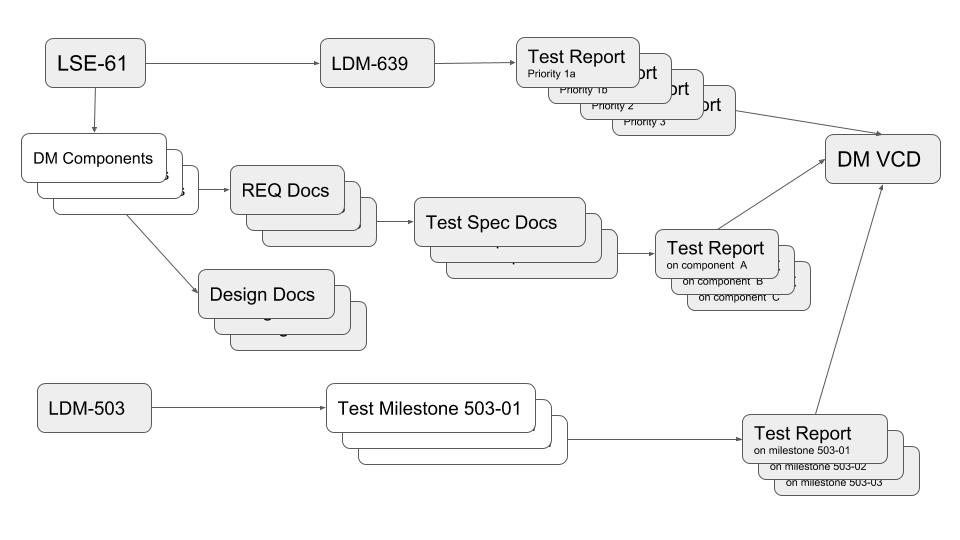
\includegraphics[width=0.9\textwidth, trim={0cm 15cm 0cm 0cm}]{DMDocTreeStructure}
                \caption{DM components as deployed during Operations. For details, refer to \citeds{LDM-148}.
                \label{fig:doctreestructure}}
        \end{center}
\end{figure}



\subsubsection{Tools}

{\bf MagicDraw}: is the tool where all modeling and requirements definition is done. System Engineering will derive the final coverage of the LSST requirement using MagicDraw, therefore the importance to have all information collected here.

{\bf Jira and Test Management Plugin}: Jira is the issue tracking system. The Test Management plugin (ATM) add verification capabilities to Jira.

{\bf Sinedia}: this is the synchronization tool between MagicDraw and Jira.

{\bf Extraction Scripts}: these scripts will permit to extract from Jira the relevant test documentation: the test specifications and the test report.


\subsubsection{Requirements and Test Objects}

{\bf Requirements}: are defined in MagicDrawi. The project CCB take care of the change control on them.
Requirements are collected in Requirements Specification documents.
Requirements are not synchronized in Jira.
Requirements are not described here in this document.

{\bf Verification Elements}: each requirement is decomposed in one or more verification element. A verification element is an aspect of the requirement that can be tested, without considering the full requirement. 
The verification elements are created in MagicDraw and sycjronized in Jira. 
Product owner are requested to update them in Jira with a proper description and other characterization paramaeter.
System Engineering will synchronize them back in MagicDraw once the update is completed.
Verification elements in Jira are implemented with a specific issue type, and are normal jira issues.

{\bf Test Cases}: are the definition of test procedure to be executed in order to prove that a related verification element is properly tested. A test case can be related with many verification elements. It is not a jira issue, but a test object provided by ATM.

{\bf Test Plans}: are test milestones to be executed in a specific moment in time in order to fulfil a specific purpose, for example validate a release or complete a verification milestone. 
The test plan is just the definition of the activity, and will not contain nor will relate directly to any test case. 
A Test Plan can be related to multiple Test Cycles and the test cycles will be related to te test cases. 
It is not a Jira issue, but a test object provided by ATM.

{\bf Test Cycles}: correspond to test runs. They are Jira objects that include multiple test cases to be executed in a specific moment in time in a specific configuration. Test Cycles are related to Test Plans, and contains list of test cases. 
It is not a Jira issue, but a test object provided by ATM.

{\bf Deviations}: in the case that it is not possible to sucessfully verify a Verification element, lets say a test case if failing,  a request for deviation can be open, asking to deviate from what agreed and approve in the requirement. 
This is implemented trough Deviation Jira issue types.

For more details on the different Jira objects and how to use them, refer to the following confluence page 
\url{https://confluence.lsstcorp.org/display/DM/DM+Test+Approach}.

Workflows on the different objects are available in SE documentation.


\subsubsection{Test Documents}

Despite all information is contained in MagicDraw and Jira, it is important to have this baselined as appropriate. This is already happening for the requirements that are captured in requirements documents, and when approved issued into Docushare.
The same shall happen for the test information, that live dynamicaly in jira.

The {\bf Test Specification} document consist on a collections of test cases that covers a specific \product{} product as defined in the document tree. These collections of test cases are available in in Jira as views in the ``LSST Verification and Validation'' project, organized in folders.

Following are the sections that characterize a test specification

\begin{itemize}
\item Introduction: includes subsections ``Objective'' and ``Scope'' to be edit and maintain manually by the autor, not in Jira, and uploade it in github.
\item Approach: to edit and maintain manually by the author, not in Jira, and uploade it in github. The relevant subsections are: ``Tasks and criteria'', `` Features to be tested'', ``Features not to be tested'', ``Pass/fail criteria'', ``Suspension criteria'', ``Naming convention''.
\item Test Case Summary: this is a summary table extracted directly from Jira that will summarize all test cases included in the test specification. Do not edit it manually, all changes need to be done in Jira.
\item Test Case Specification: this section will include all test cases details extracted automatically from Jira. Do not edit it manually, al changes need to be done in Jira.
\end{itemize}

One additional section or a first apendix should be added in order to provide proper document location on the verification elements.

Additional sections can be added in appendix.

The test specification is a living document, test cases may be added, updated or removed in Jira and new issues of the same document will be generated and uploaded in Docushare.

Note: never update a test specification in section 3 or 4, since this will be overwritten by the extraction scripts. Note also that the old naming convention is not more applicable, since the Test Case identification is assigned automatically by Jira. Existing test cases will preserve the old identification in the subject.

Taking advantage of the continuous integration process executed in Travis, the {\bf extraction scripts} will be integration in the build of the pdf in order to extract dynamically the section 3 and 4 content from Jira, on a regular basis, to be defined.


The {\bf Test Plan and Report} is the documented that will include all information related to a test campaign. 
This includes all information from the test plan and the related test runs. 
Do not edit it directly, all change need to be done in Jira.

The author need to define the structure of the document and upload it in github. The continuous integration in Travis will take case to build the document on a regular bases, to be defined.

The test plan and report scope is constrained on a single major test activity. It may only be updated, new issues, in order to included information related on a retest.
In general a new test activity, due to a new milestone or release to be tested, imply a creation of a new test plan and report.

Note that in the past this document was identified as "Test Report".
Now it is proposed to rename it to "Test Plan and Report" in order to better identify the two types of information it contains: planification of the test and report on the executed test cases. However, the document type acronym should still be DMTR. 

Note also that, the reports considered in this context are only the documents which scope is to provide information on test campaigns documented and executed using the test management infrastructure in Jira. Release characterization reports are not relevant here, unless their documentation, planification and execution will not follows these guidelines.


\subsubsection{Approval Procedure}

The approval of the test specification is already addressed via RFC as done for all the DM-CCB controlled documents.

New or updated test cases should be set to status draft, and should be put in status approved only when the test specification has been approved via RFC.
Only then the document can be regenerated with the approved test cases and uploaded in Docushare.

The approval of the test plan and report, is a bit different.
For practical reasons, the test report is completed in 2 steps:

\begin{itemize}
\item before the test execution: the plan and few information in the test cycle in jira shall be provide, in order to demonstrate that the test is ready to start. 
\item after the test execution: the document is finalized including the reports and comments on the execution of the test cases will, issues raised during the test campaign  and the a statement summarizing the global test campaign result.
\end{itemize}

Despite only the final document is relevant for deriving the global coverage of the DM requirements, it is important that both steps are consolidated and approved separately. 
Going to execute the test campaign without ensuring that everything is ready for it, it may imply the failure of the test campaign. 

The approval of the first step, comes after verification from the product owner, that all needed information are provided in Jira and therefore in the test plan and report document. 
The formality to issue the document in Docushare can be skip, but a coherent draft has to be available in DMTR-XXX.lsst.io and the status of the corresponding test plan has to be set to "approved". 
Stakeholders that may have some expectation on the activity results, like scientists, T/CAMs or others, can be involved before the approval.

The final approval of the document, after the test activity is concluded and all information is collected in Jira, should be explicitly given by whoever requested the test activity to be carried out.


A more detailed approval procedure is provided in the confluence page \url{https://confluence.lsstcorp.org/display/DM/DM+Test+Approach}.

%old section 2.3 Testing Specificatin Format

%As described in \secref{sect:reports}, test specifications consist primarily of views on the test cases managed in the Jira ``LSST Verification and Validation'' project.
%The format of these test cases has been developed in conjunction with the LSST Systems Engineering Team.
%Each test case will include:

%\begin{itemize_single}

%  \item{A description of the environment in which the test case is to be carried out (e.g.\ hardware platform) and a description of how they differ from the operational system in tests prior to final integration (e.g.\ interfaces that may be mocked without affecting that component's testing).}
%  \item{The inputs (such as data, API load, etc.) that are to be used in the test.}
%  \item{Pass-fail criteria on any metrics or other measurements.}
%  \item{How any outputs that are used to determine pass/fail (e.g.\ data or metrics) are to be published or otherwise made available.}
%  \item{A software quality assurance manifest, listing (as relevant) code repositories, configuration information, release/distribution methods and applicable documentation (such as installation instructions, developer guide, user guide etc.)} ---  this is not true.

%\end{itemize_single}

%In additon to the collection of test cases, the test specification will include:

%\begin{itemize_single}

%  \item{A list of components being tested within the scope of the test specification document.}
%  \item{A list of features in those components that are being explicitly tested.}
%  \item{The relationship between features under test and the identified requirements for the component.}

%\end{itemize_single}

\subsection{Roles and Personnel}
\label{sect:roles}

Each test specification must make clear who the \emph{tester} is.

The tester is responsible for executing the test cases following the script provided in the Jira ``LSST Verification and Validation'' project (\secref{sect:tsform}).

Testers submit details of test execution to Jira project, where it is used to log test execution and may be used to generate test reports.
The information captured in Jira will also be used to populate the Verification Control Document (see \secref{sect:approach}).

Tests and procedures will sometimes fail: a test specification may be re-run several times until it passes, but testers will log an explanation than indicates that any failures were understood (e.g.\ they were due to a fault that was fixed) or repeated sufficient times to ensure that passing the test was not transient success.
Issues which cannot be resolved by the tester in the course of carrying out the test willl be reported as ``Software Problem Reports'' (SPRs) through the \product{} ticketing system (the Jira ``Data Management'' project at the time of this document revision).
The DMCCB, or an individual designated by it, will be tasked with assessing the SPRs determining the timescale for re-executing the test procedure.

Other parties that have a relevant role in \product\ verification are identified in the appropriate sections of the document; these are involved in their primary capacity (e.g.\ the DM Systems Engineer) and so are not individually listed in this section.

\subsection{Pass/Fail Criteria}

A test case will be considered ``Passed'' when:

\begin{itemize_single}
\item{All of the test steps of the Test Case are completed; and}
\item{All open SPRs from this Test Case are considered noncritical by DMCCB.}
\end{itemize_single}

A test case will be considered ``Partially Passed'' when:

\begin{itemize_single}
\item{Only a subset of all of the test steps in the Test Case are completed and/or there remain open SPRs which are regarded as critical by the DMCCB; but}
\item{The DMCCB regards overall purpose of the test as having been met.}
\end{itemize_single}

A test case will be considered ``Failed'' when:

\begin{itemize_single}
\item{Only a subset of all of the test steps in the Test Case are completed and/or there remain open SPRs which are regarded as critical by the DMCCB; and}
\item{The DMCCB regards overall purpose of the test as not having been met.}
\end{itemize_single}

Note that in \citeds{LPM-17} science requirements are described as having a minimum specification, a design specification and a stretch goal.
While we preserve these distinctions in some DM tooling for internal tracking purposes, for the purposes of these tests, it is the design specification that is verified as having been met for a test to pass without intervention of the DMCCB.
Ultimately, if it proves impossible to satisfy a requirement at design specification, LSST Project level approval is required to accept the minimum specification.

\subsection{Constraints and Limitations}

\subsubsection{Procedural and Technical Limitations}

\begin{itemize}


  \item{The \product{} system must be verified before the complete LSST system can be completed. Verification is therefore carried out using precursor datasets~\footnote{e.g. from Hyper Suprime-Cam; \secref{LDM-503-02}}, simulated data, and --- where available --- with engineering and pre-release data from the as yet incomplete LSST system.}

  \item{Metric measurements and operational rehearsals during construction may not involve critical operational systems that are still in development. For example, while computational performance is being measured, computationally dominant algorithmic steps such as deblending and multi-epoch fitting may only be modeled, since they have not yet been implemented; operational rehearsals are done without the factory LSST workflow system; etc.}

\end{itemize}

\subsubsection{Requirements Traceability Constraints}

The \product{} verification plan is based entirely on requirements captured in the DM System Requirements (\citeds{LSE-61}).
It does not refer to higher level requirements documentation, such as the LSST System Requirements (\citeds{LSE-29}) or the Observatory System Specifications (\citeds{LSE-30}); rather, we assume that all higher level requirements have been correctly flowed down to DM.
In practice, the Systems Engineering team continues to refine the flow-down of higher level requirements and issue updates to \citeds{LSE-61}; this test plan must both anticipate and be responsive to those updates.
